\documentclass[man,floatsintext]{apa6}
\usepackage{lmodern}
\usepackage{amssymb,amsmath}
\usepackage{ifxetex,ifluatex}
\usepackage{fixltx2e} % provides \textsubscript
\ifnum 0\ifxetex 1\fi\ifluatex 1\fi=0 % if pdftex
  \usepackage[T1]{fontenc}
  \usepackage[utf8]{inputenc}
\else % if luatex or xelatex
  \ifxetex
    \usepackage{mathspec}
  \else
    \usepackage{fontspec}
  \fi
  \defaultfontfeatures{Ligatures=TeX,Scale=MatchLowercase}
\fi
% use upquote if available, for straight quotes in verbatim environments
\IfFileExists{upquote.sty}{\usepackage{upquote}}{}
% use microtype if available
\IfFileExists{microtype.sty}{%
\usepackage{microtype}
\UseMicrotypeSet[protrusion]{basicmath} % disable protrusion for tt fonts
}{}
\usepackage{hyperref}
\hypersetup{unicode=true,
            pdftitle={Drought regimens predict life history strategies in Heliophila},
            pdfauthor={J. Grey Monroe, Brian Gill, Kathryn G. Turner, \& John K. McKay},
            pdfkeywords={drought adaptation, herbaria records, Heliophila, life history
evolution, phylogeography, remote sensing},
            pdfborder={0 0 0},
            breaklinks=true}
\urlstyle{same}  % don't use monospace font for urls
\usepackage{graphicx,grffile}
\makeatletter
\def\maxwidth{\ifdim\Gin@nat@width>\linewidth\linewidth\else\Gin@nat@width\fi}
\def\maxheight{\ifdim\Gin@nat@height>\textheight\textheight\else\Gin@nat@height\fi}
\makeatother
% Scale images if necessary, so that they will not overflow the page
% margins by default, and it is still possible to overwrite the defaults
% using explicit options in \includegraphics[width, height, ...]{}
\setkeys{Gin}{width=\maxwidth,height=\maxheight,keepaspectratio}
\IfFileExists{parskip.sty}{%
\usepackage{parskip}
}{% else
\setlength{\parindent}{0pt}
\setlength{\parskip}{6pt plus 2pt minus 1pt}
}
\setlength{\emergencystretch}{3em}  % prevent overfull lines
\providecommand{\tightlist}{%
  \setlength{\itemsep}{0pt}\setlength{\parskip}{0pt}}
\setcounter{secnumdepth}{0}
% Redefines (sub)paragraphs to behave more like sections
\ifx\paragraph\undefined\else
\let\oldparagraph\paragraph
\renewcommand{\paragraph}[1]{\oldparagraph{#1}\mbox{}}
\fi
\ifx\subparagraph\undefined\else
\let\oldsubparagraph\subparagraph
\renewcommand{\subparagraph}[1]{\oldsubparagraph{#1}\mbox{}}
\fi

%%% Use protect on footnotes to avoid problems with footnotes in titles
\let\rmarkdownfootnote\footnote%
\def\footnote{\protect\rmarkdownfootnote}


  \title{Drought regimens predict life history strategies in \emph{Heliophila}}
    \author{J. Grey Monroe\textsuperscript{1,2}, Brian Gill\textsuperscript{3},
Kathryn G. Turner\textsuperscript{4}, \& John K.
McKay\textsuperscript{2}}
    \date{}
  
\shorttitle{Drought and life history}
\affiliation{
\vspace{0.5cm}
\textsuperscript{1} Graduate Degree Program in Ecology, Colorado State University, Fort Collins, CO 80521, USA\\\textsuperscript{2} College of Agriculture, Colorado State University, Fort Collins, CO 80521, USA\\\textsuperscript{3} Institute for Environment and Society, Brown University, Providence, RI 02912, USA\\\textsuperscript{4} Biology Department, Pennsylvania State University, State College, PA 16802, USA}
\keywords{drought adaptation, herbaria records, Heliophila, life history evolution, phylogeography, remote sensing }
\usepackage{csquotes}
\usepackage{upgreek}
\captionsetup{font=singlespacing,justification=justified}

\usepackage{longtable}
\usepackage{lscape}
\usepackage{multirow}
\usepackage{tabularx}
\usepackage[flushleft]{threeparttable}
\usepackage{threeparttablex}

\newenvironment{lltable}{\begin{landscape}\begin{center}\begin{ThreePartTable}}{\end{ThreePartTable}\end{center}\end{landscape}}

\makeatletter
\newcommand\LastLTentrywidth{1em}
\newlength\longtablewidth
\setlength{\longtablewidth}{1in}
\newcommand{\getlongtablewidth}{\begingroup \ifcsname LT@\roman{LT@tables}\endcsname \global\longtablewidth=0pt \renewcommand{\LT@entry}[2]{\global\advance\longtablewidth by ##2\relax\gdef\LastLTentrywidth{##2}}\@nameuse{LT@\roman{LT@tables}} \fi \endgroup}


\usepackage{lineno}

\linenumbers
\newcommand{\beginsupplement}{\setcounter{table}{0}  \renewcommand{\thetable}{S\arabic{table}} \setcounter{figure}{0} \renewcommand{\thefigure}{S\arabic{figure}}}

\authornote{

Correspondence concerning this article should be addressed to J. Grey
Monroe, 307 University Ave, Fort Collins, CO 80521. E-mail:
\href{mailto:monroejg@colostate.edu}{\nolinkurl{monroejg@colostate.edu}}}

\abstract{
\begin{center}\textbf{Summary}\end{center} \par

Explaining variation in life history strategies is an enduring goal of
evolutionary biology and ecology. Early theory predicted that for
plants, annual and perennial life histories reflect adaptation to
environments that experience alternative drought regimens. Nevertheless,
empirical support for this hypothesis from comparative analyses remains
lacking.

\par

Here, we test classic life history theory in \textit{Heliophila}
(Brassicaceae), a diverse genus of flowering plants native to Africa,
controlling for phylogeny and integrating 34 years of satellite-based
drought detection with 2,192 herbaria occurrence records.

\par

We find that the common ancestor of \textit{Heliophila} species was
likely an annual, and that perenniality and annuality have repeatedly
evolved, an estimated seven and five times, respectively. By comparing
historical drought regimens, we show that annuals occur in environments
where droughts are significantly more frequent than perennial species.
We also provide evidence that annual plants adapt to predictable drought
regimens by escaping drought prone seasons as seeds.

\par

These results yield compelling support for longstanding theoretical
predictions by revealing the importance of drought frequency and
predictability to explain plant life history. More broadly, this work
highlights scalable approaches integrating herbaria records and remote
sensing to address outstanding questions in evolutionary ecology.

}

\usepackage{amsthm}
\newtheorem{theorem}{Theorem}[section]
\newtheorem{lemma}{Lemma}[section]
\theoremstyle{definition}
\newtheorem{definition}{Definition}[section]
\newtheorem{corollary}{Corollary}[section]
\newtheorem{proposition}{Proposition}[section]
\theoremstyle{definition}
\newtheorem{example}{Example}[section]
\theoremstyle{definition}
\newtheorem{exercise}{Exercise}[section]
\theoremstyle{remark}
\newtheorem*{remark}{Remark}
\newtheorem*{solution}{Solution}
\begin{document}
\maketitle

\hypertarget{introduction}{%
\section{Introduction}\label{introduction}}

Understanding the causes and consequences of life history variation is a
longstanding goal of ecology and evolutionary biology (Cole, 1954). In
plants, life histories are especially diverse, with some species
completing their life cycle in a number of weeks to others that live for
thousands of years (Brown, 1996). Along this continuum in angiosperms an
important division exists distinguishing annuals which complete their
seed to seed life cycle within a single calendar year from perennials
which can persist over multiple years. Annual plants do not need to
survive through the full range of seasonal environmental variation and
spend at least some portion of the year as a seed where they are
relatively protected from environmental stress. In contrast, perennial
plants can continue vegetative growth over multiple years and must
survive conditions experienced during all seasons but can also benefit
from competitive advantages and, if iteroparous, multiple bouts of
reproduction. These represent fundamentally different life history
strategies and predicting their occurrence is important for community,
ecosystem, and agricultural ecology. However, the environmental factors
that explain their evolution and distributions remain empirically
unresolved (Friedman \& Rubin, 2015).

Classical theory predicts shorter life spans in environments where adult
mortality is high (Charnov \& Schaffer, 1973; Stearns, 1992; Franco \&
Silvertown, 1996). Because lack of water is perhaps the greatest threat
to survival during vegetative or reproductive growth in plants, this
theory has been extended to the hypothesis that annuality is adaptive
when it allows plants to escape drought (Schaffer \& Gadgil, 1975).
Indeed, adaptation to drought, defined as episodes of increased aridity
causing plant sress (Passioura, 1996), is often invoked as an
explanation for the success of annual species. And while a few cases are
cited where annuality appears to be more common in environments with
greater aridity (Stebbins Jr, 1952; Morishima \emph{et al.}, 1984), this
hypothesis has yet to be supported while controlling for the effect of
common ancestry (phylogeny) on life habit. In one previous study where
this question was addressed phylogenetically, (Evans \emph{et al.},
2005) annuals were not found to be associated with environments that
experience more drought. This could be explained by the relatively small
number of species studied and the reliance on a limited number of
weather stations to characterize environments, highlighting the need to
develop more scalable methods to study the geographic distributions of
traits such as life history. Thus, in this study we leverage thousands
of herbaria specimens among dozens of species and high-resolution remote
sensing to study the distributions and environmental factors potentially
driving the evolution and distribution of life history.

It is also critical to consider another dimension of drought adaptation:
the expectation that annuality is most adaptive when droughts are not
only frequent but also predictable. That is, when the frequency of
drought is particularly high during certain seasons. Such predictability
is important for selection to favor and escape strategy during those
seasons which are particularly drought prone. While there has been at
least one example of annuality associated with environments
qualitatively classified as \enquote{predictable} in a general sense
(Datson \emph{et al.}, 2008), the seasonal predictability of drought
experienced by annuals has yet to be rigorously studied. As such,
further empirical work is needed to support the model of annuality as a
mechanism of drought adaptation via escape from drought prone seasons.
Here we study herbarium collection dates to ask whether annuals indeed
exhibit evidence of an escape strategy from seasons with elevated
drought frequency.

In addition to drought escape in annuals as a mechanism of adaptation to
frequent and predictable droughts, droughts may be necessary for the
success of annuals more generally by acting as episodes of disturbance
that provide opportunities for annuals to establish and compete with
sympatric perennial species. Indeed, there is evidence that perennials
dominate in environments where disturbance events are infrequent (Rees
\& Long, 1992; Corbin \& D'Antonio, 2004; Clary, 2012). The resulting
prediction from this hypothesis is that in the absence of frequent
drought, perenniality should evolve. However, little is known about this
component of life history evolution because previous work has almost
entirely focused on the origins of annuality rather than perenniality
(Friedman \& Rubin, 2015). This highlights the need to study taxa which
have seen transitions from annual to perennial life histories as well.

Here we combine a long-term global dataset of satellite detected drought
events with metadata from natural history collections to test these
classic hypotheses within the African endemic mustard genus,
\emph{Heliophila} L. (Brassicaceae). If annuality is an adaptive
strategy allowing plants to escape drought prone seasons, then drought
frequency should predict the distribution of life history strategies
across landscapes, and annual species should be more commonly associated
with drought prone regions than perennial species. Additionally, if
perenniality offers competitive advantage in the absence of drought,
associations between life history and drought frequency should be
significant when phylogenies include transitions from annual to
perennial life history strategy. Finally, if annual species have adapted
to escape predictably drought prone seasons, observations of growing
annual species (i.e.~occurring in forms other than seed) should be rare
during seasons when drought frequency is highest. Phylogenetic
relatedness can influence tests of associations between species' traits
and their environments by confounding common environments caused by
selection from common environments caused my ancestry. (Felsenstein,
1985; Barrett \emph{et al.}, 1996). Therefore, we assessed the
relationship between life history distribution and drought frequency
while controlling for phylogeny.

\hypertarget{materials-and-methods}{%
\section{Materials and Methods}\label{materials-and-methods}}

\hypertarget{data}{%
\subsection{Data}\label{data}}

\hypertarget{data-availability}{%
\subsubsection{Data availability}\label{data-availability}}

All analyses were performed using R. All data and the source code to
produce this manuscript are available at
\url{https://github.com/greymonroe/heliophila}.

\hypertarget{life-history-data-for-heliophila}{%
\subsubsection{\texorpdfstring{Life history data for
\emph{Heliophila}}{Life history data for Heliophila}}\label{life-history-data-for-heliophila}}

\emph{Heliophila} is a genus of flowering plants endemic to southern
Africa including the Cape Floristic and Succulent Karoo Regions. These
are among the most botanically diverse environments on Earth and the
\emph{Heliophila} species occurring there are considered to be among the
most phenotypically diverse genera of the family Brassicaceae
(Mummenhoff \emph{et al.}, 2005; Mandáková \emph{et al.}, 2012). This
genus includes both perennial and annual species, and transitions
between life history strategy may have occurred multiple independent
times (Appel \& Al-Shehbaz, 1997; Mummenhoff \emph{et al.}, 2005).
Furthermore, the fine scale climatic heterogeneity of southern Africa is
ideal for studying the distribution of traits in relation to
environmental parameters (Sayre \emph{et al.}, 2013). We used life
histories reported by Mummenhoff \emph{et al.} (2005), grouping species
into annual or perennial life history categories. Perenniality was
defined as any form of perennial life history (e.g., herbs, shrubs,
mixed, etc). Because the nature of species reported with mixed traits
were unknown (i.e.~plasticity vs.~genetic variation), we classified
these species here as perennial since they can maintain vegetative
across multiple years at least to some capacity.

\hypertarget{heliophila-occurrence-records}{%
\subsubsection{\texorpdfstring{\emph{Heliophila} occurrence
records}{Heliophila occurrence records}}\label{heliophila-occurrence-records}}

To characterize the distributions of annual (studied here, n = 21) and
perennial (studied here, n = 21) \emph{Heliophila} species, all (8670)
records for the genus \emph{Heliophila} were downloaded from the Global
Biodiversity Information Facility (gbif.org) on July 21, 2018 (GBIF,
2018). Herbaria records such as these provide a rich data sources to
characterize the geographical distributions of species (Thiers, 2016;
Willis \emph{et al.}, 2017; Lang \emph{et al.}, 2018). And as they
become digitized (Soltis, 2017), herbaria collections have been used to
study relationships between trait distributions, geography, and climate
(Davis \emph{et al.}, 2015; Stropp \emph{et al.}, 2016; Wolf \emph{et
al.}, 2016; Václavı'k \emph{et al.}, 2017).

\hypertarget{sequence-data-for-phylogeny}{%
\subsubsection{Sequence data for
phylogeny}\label{sequence-data-for-phylogeny}}

An alignment of ITS I and II sequences for 21 annual and 21 perennial
\emph{Heliophila} species was obtained from the authors of Mandáková
\emph{et al.} (2012). Individual ITS I and II sequences for
\emph{Aethionema grandiflorum, Alliaria petiolata, Cardamine matthioli,
Chamira circaeoides}, and \emph{Rorippa amphibia} were downloaded from
Genbank.

\hypertarget{satellite-detected-drought-data}{%
\subsubsection{Satellite-detected drought
data}\label{satellite-detected-drought-data}}

Remotely sensed data is a powerful tool for characterizing seasonal
patterns in drought because it is less limited in spatial and temporal
scope and resolution than weather stations or field observations
(AghaKouchak \emph{et al.}, 2015). From an ecological perspective,
droughts are best defined as episodes of plant stress caused by elevated
aridity (Passioura, 1996). Thus remote sensing offers the additional
benefit for studying drought as an agent of natural selection because
plant stress caused by drought can be observed from space (Kogan,
1995a). The remotely sensed Vegetative Health Index (VHI) is one such
metric, which detects landscape scale reductions in plant cover and
temperature conditions characteristic of drought (Kogan, 2001).
Generated from data collected by NOAA AVHRR satellites since 1981, the
VHI is a composite index combining Normalized Difference Vegetation
Index (NDVI) derived quantification of vegetative stress (Vegetative
Condition Index - VCI) with temperature stress indicated by anomalies in
thermal spectra (Temperature Condition Index - TCI). These indices were
developed to create an unbiased quantification of drought across
ecosystem types. The VHI of year \(y\) during week \(w\) of \([1,52]\)
at pixel \(i\) is derived from the following equations, where \(n\) is
the number of years observed.

\[VCI_{y,w,i} = 100\frac{NDVI_{y,w,i} - NDVI_{min,w,i}}{NDVI_{max,w,i} - NDVI_{min,w,i}}\]

Low values of VCI indicate episodes when plant cover is particularly low
for a given location during a given time of the year. Thus, it controls
for the location and season in quantifying plant stress.

\[TCI_{y,w,i} = 100\frac{T_{max,w,i}-T_{y,w,i}}{T_{max,w,i} - T_{min,w,i}}\]
Similarly, low TCI values indicate episdoes of high thermal stress shown
to be negatively correlated with precipitation and soil moisture
(AghaKouchak \emph{et al.}, 2015).

\[VHI_{y,w,i} = 0.5(VCI_{y,w,i}) + 0.5(TCI_{y,w,i})\] By combining VCI
and TCI, the VHI distinguishes drought from other forms of vegetative
stress (Kogan, 1995b). The use of the VHI to detect drought has been
validated globally and across ecosystem types (AghaKouchak \emph{et
al.}, 2015), including in southern Africa, the focal region of this
study (e.g.~Figure \ref{fig:mapsdroughtexamples}). To date, the VHI has
most often been applied for evaluating drought risk for agricultural
research (e.g., Rojas \emph{et al.}, 2011; Kogan \emph{et al.}, 2016).
But it also presents a tool to study seasonal patterns in the frequency
of drought across environments and to test hypotheses about the effect
of drought on ecological and evolutionary processes (Kerr \& Ostrovsky,
2003). As such, the VHI has been applied recently to study drought
related ecology of natural species and proven useful for predicting
intraspecific variation in drought tolerance traits and genes (Mojica
\emph{et al.}, 2016; Dittberner \emph{et al.}, 2018; Monroe \emph{et
al.}, 2018b). Here, we accessed VHI data at \(16km^2\) resolution from
1981 to 2015
(\url{https://www.star.nesdis.noaa.gov/smcd/emb/vci/VH/vh_ftp.php}) to
characterize the seasonal drought frequencies experienced by annual and
perennial \emph{Heliophila} species across their native range of
southern Africa.

\hypertarget{analyses}{%
\subsection{Analyses}\label{analyses}}

\hypertarget{drought-frequency-calculations}{%
\subsubsection{Drought frequency
calculations}\label{drought-frequency-calculations}}

To characterize drought regimens across the distributions of annual and
perennial species of \emph{Heliophila}, we calculated drought during
different seasons at the location of observations for \emph{Heliophila}
records using the VHI. Specifically, we created maps of the frequencies
of observing drought conditions between years (VHI\textless{}40, NOAA)
during the winter (quarter surrounding winter solstice), spring (quarter
surrounding spring equinox), summer (quarter surrounding summer
solstice) and fall (quarter surrounding fall equinox) from 1981 to 2015
across the range of \emph{Heliophila}. From these maps, the drought
frequency (the number of times drought is observed divided by the total
number of years, 34) during the winter, spring, summer, and fall were
extracted for the locations of all GBIF records.

\hypertarget{filtering-of-occurrence-records}{%
\subsubsection{Filtering of occurrence
records}\label{filtering-of-occurrence-records}}

To avoid instances with spurious location data, we filtered raw GBIF
records by restricting our analyses to include only:

\begin{itemize}
\tightlist
\item
  records for species with reported life history\\
\item
  records with geospatial data\\
\item
  records without known geospatial coordinate issues (i.e., coordinates
  reported are those of herbarium)\\
\item
  records from collection sites classified as land pixels in the VHI
  dataset\\
\item
  records from Africa (to exclude locations of cultivation)
\item
  records without duplicates (i.e., identical species, location,
  collection date)
\end{itemize}

\hypertarget{phylogeny-construction-and-ancestral-state-estimation}{%
\subsubsection{Phylogeny construction and ancestral state
estimation}\label{phylogeny-construction-and-ancestral-state-estimation}}

Outgroup ( \emph{Aethionema grandiflorum, Alliaria petiolata, Cardamine
matthioli, Chamira circaeoides}, and \emph{Rorippa amphibia}) and
ingroup \emph{Heliophila} ITS I and II sequences were aligned using
MAFFT (Katoh \emph{et al.}, 2002) with strategy G-INS-I, offset value
0.1, and all other options set as default. The \(GTR + \Gamma\) model of
nucleotide substitution was determined to best fit the data based on AIC
using jModelTest2 (Guindon \& Gascuel, 2003; Darriba \emph{et al.},
2012). A maximum clade credibility tree with branch lengths as relative
time was estimated by summarizing data from six runs of 100,000,000
generations of Bayesian Markov chain Monte Carlo conducted in BEAST 2
(Bouckaert \emph{et al.}, 2014). Model selection and phylogenetic
analyses were conducted through the CIPRES Science Gateway (Miller
\emph{et al.}, 2010). Ancestral state estimation was performed in R
using the package phytools (Revell, 2012) to generate 10,000 stochastic
character maps simulated under an equal rates model of character
evolution for the trait life habit (annual or perennial).

\hypertarget{comparison-of-drought-frequency-between-annual-and-perennial-species}{%
\subsubsection{Comparison of drought frequency between annual and
perennial
species}\label{comparison-of-drought-frequency-between-annual-and-perennial-species}}

To evaluate the hypothesis that annual and perennial life history
strategies reflect adaptations to alternative drought regimens, we
tested the corresponding prediction that the observed distributions of
annual and perennial \emph{Heliophila} species would be significantly
associated with historic drought frequency. We tested for a relationship
between drought frequency and life history, season, and their
interaction by analysis of variance while including species as a random
effect using the lme4 package in R ({\textbf{???}}) and compared annuals
and perennials using by Tukey adjusted post-hoc contrasts. We next
calculated the mean drought frequency during the winter, spring, summer
and fall for each species. Because shared evolutionary history of
closely related species can lead to spurious associations between traits
and environments (Felsenstein, 1985), we tested for a relationship
between life history strategy and drought frequency while controlling
for phylogeny using phylogenetic logistic regression (Ives \& Garland,
2010). This statistical approach is designed to control for the
confounding effects of common ancestry's influence on demographic
features such as geospatial relationships when addressing hypotheses
about the role of natural selection on trait distributions.

\hypertarget{collection-dates}{%
\subsubsection{Collection dates}\label{collection-dates}}

To test the hypothesis that annual species have adapted to escape
drought prone seasons as seeds, collection dates for herbarium specimens
were compared between annual and perennial species. Comparisons of
distributions were made by Two-sample Kolmogorov-Smirnov test and
Barlett variance test.

\hypertarget{results}{%
\section{Results}\label{results}}












\begin{figure}[!h]
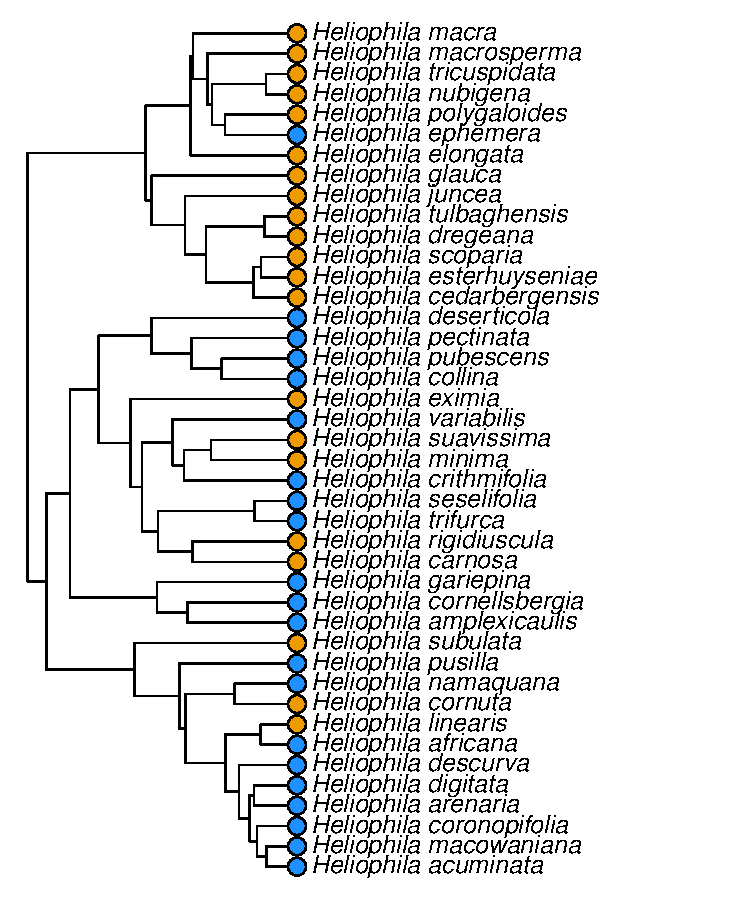
\includegraphics[width=\textwidth]{../figures/phylogeny} \caption{Species and examples of herbaria specimens of
\emph{Heliophila} (a) Phylogeny and life history strategies of species
studied. Orange circles at branch tips mark annual species and blue
circles mark perennial species. At internal nodes, pie charts indicate
the estimated posterior probability of being annual versus perennial.
Example herbaria specimens accessed via GBIF of (a) \emph{H. minima},
(b) \emph{H. deserticola}, (c) \emph{H. coronopifolia} and (d) \emph{H.
ephemera}. Images (b,d,e) courtesy of The Bavarian Natural History
Collections (CC BY-SA 4.0) and (c) The London Natural History Museum (CC
BY 4.0). Links to images are found in the supplement.}\label{fig:phylogeny}
\end{figure}








\begin{figure}[!h]
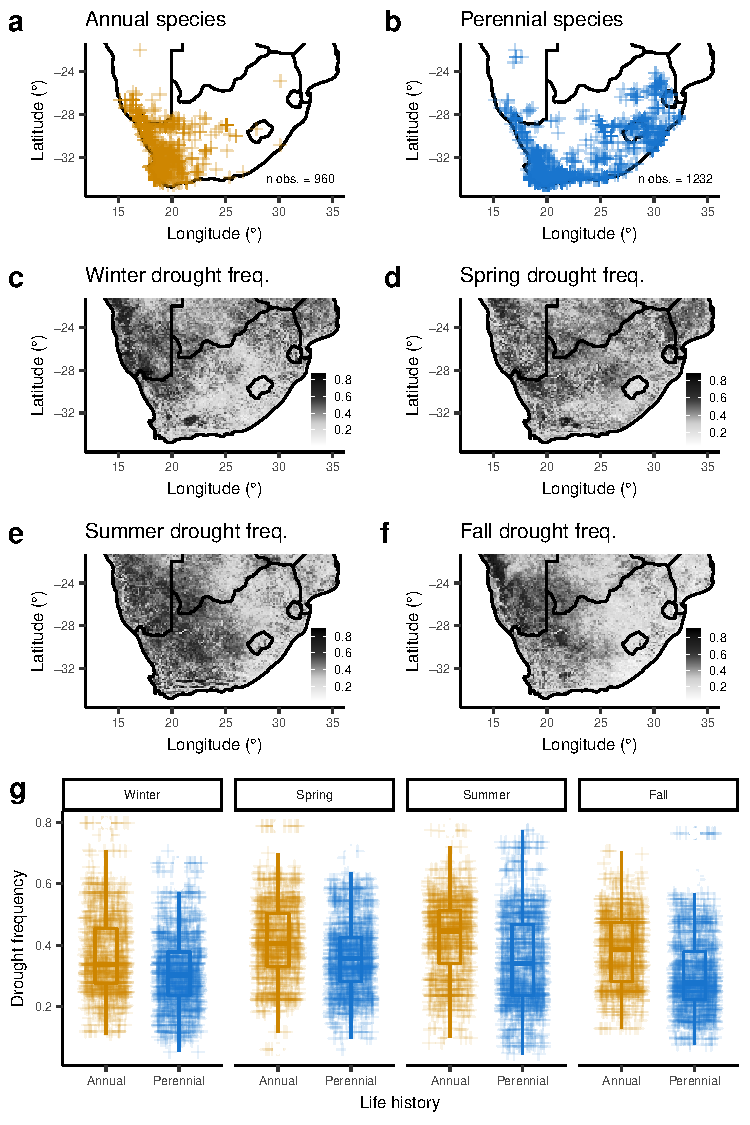
\includegraphics[width=\textwidth]{../figures/maps_boxplots} \caption{Locations of occurrence records of (a) annual and (b)
perennial \emph{Heliophila.} Drought frequency during the (c) winter,
(d) spring, (e) summer and (f) fall detected using the VHI. (g) Drought
frequencies during each season at the observation locations of annual
and perennial \emph{Heliophila} (Post-hoc contrasts annuals and
perennials from ANOVA, ** = p \textless{} 0.01).}\label{fig:mapsboxplots}
\end{figure}

The topology of the estimated \emph{Heliophila} phylogeny was consistent
with previous studies (Mummenhoff \emph{et al.}, 2005; Mandáková
\emph{et al.}, 2012). Based on 10,000 stochastic character maps
simulated under an equal rates model of character evolution in life
history, an average of approximately seven changes from annual to
perennial and five changes from perennial to annual are observed per
stochastic character map (Figure \ref{fig:phylogeny}a). These results
suggest that the ancestral state of \emph{Heliophila} was annual and
that both character states have arisen independently mutliple times.

Out of 8670 \emph{Heliophila} GBIF records, 6634 were for species with
reported life history (Mummenhoff \emph{et al.}, 2005), 2856 had
geospatial data, 2833 did not have geospatial issues, 2684 were located
on pixels classified as land having drought measurements, 2543 were
located in Africa, 2192 were not duplicated. Thus, after all filtering
steps, 2192 records for 42 species (Figure \ref{fig:phylogeny}, Table
\ref{tab:speciesmeanstable}) passed for further analyses. The number of
samples varied between species, with a mean of 52.19 samples per
species. \emph{H. rigidiuscula} had the most records, 201, and \emph{H.
cornellsbergia} the fewest, 2 (Table \ref{tab:speciesmeanstable}).

There were clear visual differences between the distributions of the 960
annual and the 1232 perennial \emph{Heliophila} observation records (see
Figure \ref{fig:speciesmaps} for maps of individual species). While
annual species were generally found in the western regions of South
Africa and Namibia, primarily in the Cape Floristic Region and Succulent
Karoo (Figure \ref{fig:mapsboxplots}a), the occurrence of perennials
extended to the southern and eastern coast of South Africa (Figure
\ref{fig:mapsboxplots}b).

The frequency of drought varied considerably across the ranges of
\emph{Heliophila} species (Figure \ref{fig:mapsboxplots}c-f). This
heterogeneity is expected, given that this is one of the most
climatically diverse regions of the Earth (Sayre \emph{et al.}, 2013).
It is worth noting the east to west cline in drought frequency observed
during the summer, which distinguishes the high drought frequency of the
Kalahari Sands and Namid Desert phytogeographic regions from the low
drought frequency of the Drakensberg Mountains and Coastal Zambesian
phytogeographic regions. In the Cape phytogeographic region there was
finer scale heterogeneity in drought frequency during the summer.

We found that the frequency of drought was significantly higher at the
locations of occurrence records for annual species. When comparing
across all occurrence records (all records rather than species means,
Figure \ref{fig:mapsboxplots}g), a mixed-model analysis of variance
which included species as random effect revealed a significant
relationship between drought frequency and life history (p \textless{}
0.01), season (p \textless{} 0.01) and their interaction (p \textless{}
0.01) (Table \ref{tab:anovatable}). Post-hoc contrasts showed that the
frequency of drought was significantly higher at the location of annuals
during the summer (z ratio = 3.93, p = \textless{} 0.01), and fall (z
ratio = 4.06, p \textless{} 0.01). Because a comparison across all
occurrence records does not account for variation in the number of
records per species (Table \ref{tab:speciesmeanstable}) or species
relatedness (Figure \ref{fig:phylogeny}a), we also tested whether mean
drought frequency values of each species were significantly different
between annuals and perennials using phylogenetic logistic regression.
We found that the mean drought frequencies were significantly higher
(\(\alpha = 0.05\)) in annual species during the spring, summer, and
fall (Table \ref{tab:modelstable}, Figure \ref{fig:lineplots}a,b). These
findings indicate that common ancestry alone does not explain
differences in the drought frequencies experienced between the
environments of annual and perennial \emph{Heliophila}.

\begin{table}[tbp]
\begin{center}
\begin{threeparttable}
\caption{\label{tab:modelstable}Phylogenetic logistic regressions between life history, and the mean drought frequency observed at specimen sites of Heliophila species the winter, spring, summer, and fall.}
\begin{tabular}{lll}
\toprule
Predictor & \multicolumn{1}{c}{Estimate} & \multicolumn{1}{c}{P}\\
\midrule
Intercept & 0.7231 & 0.6636\\
Winter drought freq. & -1.5452 & 0.7274\\ \midrule
Intercept & 5.0107 & 0.0534\\
Spring drought freq. & -12.9014 & 0.0464\\ \midrule
Intercept & 7.7093 & 0.0054\\
Summer drought freq. & -19.9056 & 0.0042\\ \midrule
Intercept & 7.0162 & 0.0082\\
Fall drought freq. & -20.8174 & 0.0067\\ \midrule
\bottomrule
\addlinespace
\end{tabular}
\begin{tablenotes}[para]
\normalsize{\textit{Note.} Annual species were scored as 0 and perennial species as 1.}
\end{tablenotes}
\end{threeparttable}
\end{center}
\end{table}











\begin{figure}[!h]
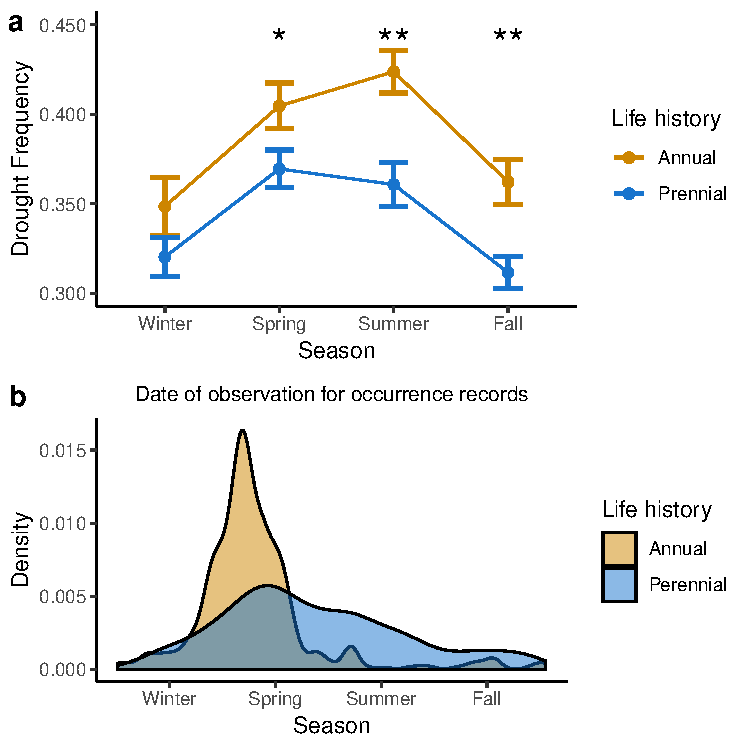
\includegraphics[width=\textwidth]{../figures/line_and_dates} \caption{(a) Comparison (mean +- SE) of drought frequency across
seasons calculated at the occurrence locations of GBIF records of annual
and perennial species of \emph{Heliophila}. (b) Results from
phylogenetic logistic regression, where the line shows the model fit and
* = p \textless{} 0.05, ** = p \textless{} 0.01. Annuals were scored as
0 and perennials as 1. (c) Collection dates of GBIF records of annual
and perennial species of \emph{Heliophila} in relation to the
photoperiodic calendar where day 1 is intermediate to the fall equinox
and winter solstice.}\label{fig:lineplots}
\end{figure}

The preceding results indicate that annual species are found in
environments where droughts are significantly more frequent, especially
in the summer and fall. Classic life history theory hypothesizes that
annuality reflects adaptation to such environments because it allows
species to escape predictable stressful conditions. If this is the case,
we would expect that annuals spend the drought prone seasons of summer
and fall as seeds. To test this hypothesis, we compared the dates of
occurrence records between annual and perennial \emph{Heliophila}
species. The distributions reveal a considerable difference in the
timing of observation of these two life histories. In comparison to
perennials, which appear to be collected throughout the year, annuals
are almost exclusively observed during the winter and spring (Figure
\ref{fig:lineplots}b). The differences between the distribution of
collection dates were significant by all tests (ks.test D = 0.25, p
\textless{} 0.01; bartlett.test K2 = 503.18, p \textless{} 0.01) This is
consistent with a model of life history in which annual species flower
in the spring, set seed, senesce, and die before the summer. Thus, these
annual species are likely to remain dormant during the summer and fall,
when drought is the strongest predictor of the distributions of annual
and perennial life histories (Figure \ref{fig:lineplots}a).

\hypertarget{discussion}{%
\section{Discussion}\label{discussion}}

To test the hypothesis that annual and perennial plants reflect
adaptation to alternative drought environments we examined the landscape
distribution of life history strategies in the large and diverse mustard
genus, \emph{Heliophila}. Using metadata of 2192 occurrence records and
a 34 year dataset of satellite-detected droughts, we tested the
prediction that annual species are more often observed in drought-prone
locations than perennial species, when controlling for phylogenetic
relatedness. We found that drought frequency is significantly different
between the distributions of annual and perennial species, with annuals
being found in environments with more frequent drought, and that this
signal is strongest during the seasons when annuals are likely escaping
via seed dormancy. These results remain significant while controlling
for the phylogenetic relationships of \emph{Heliophila} species,
yielding support for the role that natural selection has played in
driving contemporary distributions of these alternatives strategies in
relation to drought regimens.

We cannot eliminate the possibility that confounding traits or
environmental variables are the causative factors explaining variation
in the distributions of annual and perennial species. Nevertheless,
these results provide quantitative support for the classic prediction
that annual species are found in environments that experience more
frequent drought than perennial species, building on previous
investigations of associations between life history and climate
(Morishima \emph{et al.}, 1984; Evans \emph{et al.}, 2005; Datson
\emph{et al.}, 2008; Cruz-Mazo \emph{et al.}, 2009). To our knowledge
this is the first study to demonstrate a significant association between
life history and drought in a phylogenetic context informed by large
scale species distribution data and long term drought detection.

Unfortunately, herbarium collections and their associated data do not
represent systematic or random sampling of a species distribution.
Significant biases in collecting exist, which we have not necessarily
controlled for here, and may have some effect on our findings, such as a
bias toward collecting near roads or near the locations of natural
history collections (Daru \emph{et al.}, 2018). Future research will
benefit from systematic sampling efforts to avoid these noted biases.
However, the ecosystems of southern Africa include several biodiversity
hotspots and are among the most botanically well sampled regions on
Earth (Daru \emph{et al.}, 2018), suggesting that this may currently be
the optimal region for our analyses of life history distribution.
Indeed, we were able to use 2192 occurrence records to study 42 species,
which represents a significant advance over relying on personal
observations to characterize species distributions.

These findings empirically support classical theoretical predictions
about the adaptive value of annual and perennial life history
strategies. Taken together, they suggest that in \emph{Heliophila},
annual species are adapted to environments with predictable droughts by
escaping drought prone seasons during the dormant seed phase of their
life cycle. They also suggest that perenniality is adaptive in
environments where droughts are less frequent. While most previous work
has focused on describing the evolutionary origins of annuality (Barrett
\emph{et al.}, 1996; Conti \emph{et al.}, 1999; Andreasen \& Baldwin,
2001; Verboom \emph{et al.}, 2004; Friedman \& Rubin, 2015) there are at
least a few other cases where perenniality appears to have arisen from
an annual ancestor (Bena \emph{et al.}, 1998; Tank \& Olmstead, 2008).
And while early theory predicted selection for annuality when adult
mortality is high (Stearns, 1992), we also find evidence that
perenniality could be explained by reduced frequency of drought. This is
supported by the theoretical prediction that perenniality is
advantageous in stable habitats. The phylogeny reveals several
transitions from annual to perennial life history (Figure
\ref{fig:phylogeny}a) and the distributions of perennial
\emph{Heliophila} extend into regions where drought frequency is low
(Figure \ref{fig:mapsboxplots}b, Figure \ref{fig:speciesmaps}).
Perennials may be able to out compete annual relatives in environments
where the infrequency of drought favors strategies that allow plants to
benefit from growth over many seasons. This also suggests that annuals
rely on drought as a source of disturbance for seedling recruitment when
competing with perennials (Corbin \& D'Antonio, 2004). Indeed, no annual
species were observed in the low drought regions of eastern South Africa
(Figure \ref{fig:mapsboxplots}, Figure \ref{fig:speciesmaps}).

These findings suggest that species with locally adaptive life history
strategies could be threatened by rapidly changing drought regimens
(Dai, 2011). In light of the findings here, forecasted reductions in
rainfall across eastern South Africa (Service \& Comission, 2017) could
be particularly impactful to plant community compositions. Here we found
that this region is currently dominated by derived perennial species of
\emph{Heliophila}. However, a scenario in which droughts become more
frequent in this region may allow for the establishment of annuals. Such
changes in selection patterns and shifts in plant functional diversity
could have impacts on ecosystem functioning and processes such as carbon
cycling (Garnier \emph{et al.}, 1997; Roumet \emph{et al.}, 2006; Monroe
\emph{et al.}, 2018a). Furthermore, the changes in frequency of drought
may be an important factor when considering the use of perennial
cropping systems (Parry \emph{et al.}, 2005; Lelièvre \& Volaire, 2009).

In conclusion, we find strong support for classic life history theory
that predicts that annuality is adaptive in environments with frequency
and predictable droughts. We report evidence consistent with a life
history model in annuals in which they escape drought prone seasons
during the seed phase of their life cycle. Finally, we find evidence
that the distributions of perennial lineages may indicate a competitive
advantage in areas where droughts are infrequent. More broadly, this
work highlights the irreplaceable value of natural history collections
and demonstrates the power of combining such information with large
scale remote sensing data to address outstanding classic hypotheses in
ecology and evolution.

\hypertarget{acknowledgments}{%
\section{Acknowledgments}\label{acknowledgments}}

We thank Jesse Lasky, members of the Sloan lab, and three anonymous
reviewers for generous feedback that improved the quality of this work.
This research was supported by NSF Award 1701918 and USDA-NIFA Award
2014-38420-21801 to JGM.

\hypertarget{author-contributions}{%
\section{Author contributions}\label{author-contributions}}

JGM, BG, KGT and JKM contributed to the design of the research,
interpretation, and writing the manuscript. JGM, BG, and KGT contributed
to the performance of the research and data analysis.

\hypertarget{references}{%
\section{References}\label{references}}

\begingroup
\setlength{\parindent}{-0.5in}
\setlength{\leftskip}{0.5in}

\hypertarget{refs}{}
\leavevmode\hypertarget{ref-aghakouchak2015remote}{}%
\textbf{\textnormal{AghaKouchak A}, \textnormal{Farahmand A},
\textnormal{Melton F}, \textnormal{Teixeira J}, \textnormal{Anderson M},
\textnormal{Wardlow BD}, \textnormal{Hain C}}. \textbf{2015}. Remote
sensing of drought: Progress, challenges and opportunities.
\emph{Reviews of Geophysics} \textbf{53}: 452--480.

\leavevmode\hypertarget{ref-andreasen2001unequal}{}%
\textbf{\textnormal{Andreasen K}, \textnormal{Baldwin BG}}.
\textbf{2001}. Unequal evolutionary rates between annual and perennial
lineages of checker mallows (sidalcea, malvaceae): Evidence from
18S--26S rDNA internal and external transcribed spacers. \emph{Molecular
Biology and Evolution} \textbf{18}: 936--944.

\leavevmode\hypertarget{ref-appel1997generic}{}%
\textbf{\textnormal{Appel O}, \textnormal{Al-Shehbaz IA}}.
\textbf{1997}. Generic limits and taxonomy of hornungia, pritzelago, and
hymenolobus (brassicaceae). \emph{Novon}: 338--340.

\leavevmode\hypertarget{ref-barrett1996comparative}{}%
\textbf{\textnormal{Barrett SCH}, \textnormal{Harder LD},
\textnormal{Worley AC}}. \textbf{1996}. The comparative biology of
pollination and mating in flowering plants. \emph{Phil. Trans. R. Soc.
Lond. B} \textbf{351}: 1271--1280.

\leavevmode\hypertarget{ref-bena1998molecular}{}%
\textbf{\textnormal{Bena G}, \textnormal{Lejeune B},
\textnormal{Prosperi J-M}, \textnormal{Olivieri I}}. \textbf{1998}.
Molecular phylogenetic approach for studying life-history evolution: The
ambiguous example of the genus medicago l. \emph{Proceedings of the
Royal Society of London B: Biological Sciences} \textbf{265}:
1141--1151.

\leavevmode\hypertarget{ref-bouckaert2014beast}{}%
\textbf{\textnormal{Bouckaert R}, \textnormal{Heled J},
\textnormal{Kühnert D}, \textnormal{Vaughan T}, \textnormal{Wu C-H},
\textnormal{Xie D}, \textnormal{Suchard M}, \textnormal{Rambaut A},
\textnormal{Drummond A}}. \textbf{2014}. BEAST 2: A software platform
for bayesian evolutionary analysis. \emph{PLoS Computational Biology}
\textbf{10}: doi:10.1371/journal.pcbi.1003537.

\leavevmode\hypertarget{ref-brown1996oldlist}{}%
\textbf{\textnormal{Brown PM}}. \textbf{1996}. OLDLIST: A database of
maximum tree ages. \emph{Tree rings, environment, and humanity.
Radiocarbon} \textbf{1996}: 727--731.

\leavevmode\hypertarget{ref-charnov1973life}{}%
\textbf{\textnormal{Charnov EL}, \textnormal{Schaffer WM}}.
\textbf{1973}. Life-history consequences of natural selection: Cole's
result revisited. \emph{The American Naturalist} \textbf{107}: 791--793.

\leavevmode\hypertarget{ref-clary2012determinants}{}%
\textbf{\textnormal{Clary J}}. \textbf{2012}. Determinants of perennial
and annual grass distribution in mediterranean-climate california.
\emph{Plant Ecology} \textbf{213}: 1203--1208.

\leavevmode\hypertarget{ref-cole1954population}{}%
\textbf{\textnormal{Cole LC}}. \textbf{1954}. The population
consequences of life history phenomena. \emph{The Quarterly Review of
Biology} \textbf{29}: 103--137.

\leavevmode\hypertarget{ref-conti1999phylogenetic}{}%
\textbf{\textnormal{Conti E}, \textnormal{Soltis DE}, \textnormal{Hardig
TM}, \textnormal{Schneider J}}. \textbf{1999}. Phylogenetic
relationships of the silver saxifrages (saxifraga, sect. Ligulatae
haworth): Implications for the evolution of substrate specificity, life
histories, and biogeography. \emph{Molecular Phylogenetics and
Evolution} \textbf{13}: 536--555.

\leavevmode\hypertarget{ref-corbin2004competition}{}%
\textbf{\textnormal{Corbin JD}, \textnormal{D'Antonio CM}}.
\textbf{2004}. Competition between native perennial and exotic annual
grasses: Implications for an historical invasion. \emph{Ecology}
\textbf{85}: 1273--1283.

\leavevmode\hypertarget{ref-cruz2009molecular}{}%
\textbf{\textnormal{Cruz-Mazo G}, \textnormal{Buide M},
\textnormal{Samuel R}, \textnormal{Narbona E}}. \textbf{2009}. Molecular
phylogeny of scorzoneroides (asteraceae): Evolution of heterocarpy and
annual habit in unpredictable environments. \emph{Molecular
phylogenetics and evolution} \textbf{53}: 835--847.

\leavevmode\hypertarget{ref-dai2011drought}{}%
\textbf{\textnormal{Dai A}}. \textbf{2011}. Drought under global
warming: A review. \emph{Wiley Interdisciplinary Reviews: Climate
Change} \textbf{2}: 45--65.

\leavevmode\hypertarget{ref-darriba2012jmodeltest}{}%
\textbf{\textnormal{Darriba D}, \textnormal{Taboada G},
\textnormal{Doallo R}, \textnormal{Posada D}}. \textbf{2012}. JModelTest
2: More models, new heuristics and parallel computing. \emph{Nature
Methods} \textbf{9}: 772.

\leavevmode\hypertarget{ref-daru2018widespread}{}%
\textbf{\textnormal{Daru BH}, \textnormal{Park DS}, \textnormal{Primack
RB}, \textnormal{Willis CG}, \textnormal{Barrington DS},
\textnormal{Whitfeld TJ}, \textnormal{Seidler TG}, \textnormal{Sweeney
PW}, \textnormal{Foster DR}, \textnormal{Ellison AM} \emph{et al.}}
\textbf{2018}. Widespread sampling biases in herbaria revealed from
large-scale digitization. \emph{New Phytologist} \textbf{217}: 939--955.

\leavevmode\hypertarget{ref-datson2008climate}{}%
\textbf{\textnormal{Datson P}, \textnormal{Murray B},
\textnormal{Steiner K}}. \textbf{2008}. Climate and the evolution of
annual/perennial life-histories in nemesia (scrophulariaceae).
\emph{Plant Systematics and Evolution} \textbf{270}: 39--57.

\leavevmode\hypertarget{ref-davis2015herbarium}{}%
\textbf{\textnormal{Davis CC}, \textnormal{Willis CG},
\textnormal{Connolly B}, \textnormal{Kelly C}, \textnormal{Ellison AM}}.
\textbf{2015}. Herbarium records are reliable sources of phenological
change driven by climate and provide novel insights into species'
phenological cueing mechanisms. \emph{American Journal of Botany}
\textbf{102}: 1599--1609.

\leavevmode\hypertarget{ref-dittberner2018natural}{}%
\textbf{\textnormal{Dittberner H}, \textnormal{Korte A},
\textnormal{Mettler-Altmann T}, \textnormal{Weber A}, \textnormal{Monroe
G}, \textnormal{Meaux J de}}. \textbf{2018}. Natural variation in
stomata size contributes to the local adaptation of water-use efficiency
in arabidopsis thaliana. \emph{bioRxiv}: 253021.

\leavevmode\hypertarget{ref-evans2005climate}{}%
\textbf{\textnormal{Evans ME}, \textnormal{Hearn DJ}, \textnormal{Hahn
WJ}, \textnormal{Spangle JM}, \textnormal{Venable DL}}. \textbf{2005}.
Climate and life-history evolution in evening primroses (oenothera,
onagraceae): A phylogenetic comparative analysis. \emph{Evolution}
\textbf{59}: 1914--1927.

\leavevmode\hypertarget{ref-felsenstein1985phylogenies}{}%
\textbf{\textnormal{Felsenstein J}}. \textbf{1985}. Phylogenies and the
comparative method. \emph{American Naturalist} \textbf{125}: 1--15.

\leavevmode\hypertarget{ref-franco1996life}{}%
\textbf{\textnormal{Franco M}, \textnormal{Silvertown J}}.
\textbf{1996}. Life history variation in plants: An exploration of the
fast-slow continuum hypothesis. \emph{Phil. Trans. R. Soc. Lond. B}
\textbf{351}: 1341--1348.

\leavevmode\hypertarget{ref-friedman2015all}{}%
\textbf{\textnormal{Friedman J}, \textnormal{Rubin MJ}}. \textbf{2015}.
All in good time: Understanding annual and perennial strategies in
plants. \emph{American journal of botany} \textbf{102}: 497--499.

\leavevmode\hypertarget{ref-garnier1997specific}{}%
\textbf{\textnormal{Garnier E}, \textnormal{Cordonnier P},
\textnormal{Guillerm J-L}, \textnormal{Sonié L}}. \textbf{1997}.
Specific leaf area and leaf nitrogen concentration in annual and
perennial grass species growing in mediterranean old-fields.
\emph{Oecologia} \textbf{111}: 490--498.

\leavevmode\hypertarget{ref-gbifdownload}{}%
\textbf{\textnormal{GBIF}}. \textbf{2018}. GBIF occurrence download.

\leavevmode\hypertarget{ref-guindon2003a}{}%
\textbf{\textnormal{Guindon S}, \textnormal{Gascuel O}}. \textbf{2003}.
A simple, fast and accurate method to estimate large phylogenies by
maximum-likelihood. \emph{Systematic Biology} \textbf{52}: 696--704.

\leavevmode\hypertarget{ref-ives2010phylogenetic}{}%
\textbf{\textnormal{Ives A}, \textnormal{Garland T}}. \textbf{2010}.
CPhylogenetic logistic regression for binary dependent variables.
\emph{Systematic Biology} \textbf{59}: 9--26.

\leavevmode\hypertarget{ref-katoh2002mafft}{}%
\textbf{\textnormal{Katoh}, \textnormal{Misawa}, \textnormal{Kuma},
\textnormal{Miyata}}. \textbf{2002}. MAFFT: A novel method for rapid
multiple sequence alignment based on fast fourier transform.
\emph{Nucleic Acids Research} \textbf{30}: 3059--3066.

\leavevmode\hypertarget{ref-kerr2003space}{}%
\textbf{\textnormal{Kerr JT}, \textnormal{Ostrovsky M}}. \textbf{2003}.
From space to species: Ecological applications for remote sensing.
\emph{Trends in ecology \& evolution} \textbf{18}: 299--305.

\leavevmode\hypertarget{ref-kogan1995droughts}{}%
\textbf{\textnormal{Kogan FN}}. \textbf{1995a}. Droughts of the late
1980s in the united states as derived from noaa polar-orbiting satellite
data. \emph{Bulletin of the American Meteorological Society}
\textbf{76}: 655--668.

\leavevmode\hypertarget{ref-kogan1995application}{}%
\textbf{\textnormal{Kogan FN}}. \textbf{1995b}. Application of
vegetation index and brightness temperature for drought detection.
\emph{Advances in space research} \textbf{15}: 91--100.

\leavevmode\hypertarget{ref-kogan2001operational}{}%
\textbf{\textnormal{Kogan FN}}. \textbf{2001}. Operational space
technology for global vegetation assessment. \emph{Bulletin of the
American Meteorological Society} \textbf{82}: 1949--1964.

\leavevmode\hypertarget{ref-kogan2016modelling}{}%
\textbf{\textnormal{Kogan F}, \textnormal{Guo W}, \textnormal{Strashnaia
A}, \textnormal{Kleshenko A}, \textnormal{Chub O}, \textnormal{Virchenko
O}}. \textbf{2016}. Modelling and prediction of crop losses from noaa
polar-orbiting operational satellites. \emph{Geomatics, Natural Hazards
and Risk} \textbf{7}: 886--900.

\leavevmode\hypertarget{ref-lang2018using}{}%
\textbf{\textnormal{Lang PL}, \textnormal{Willems FM},
\textnormal{Scheepens J}, \textnormal{Burbano HA}, \textnormal{Bossdorf
O}}. \textbf{2018}. \emph{Using herbaria to study global environmental
change}. PeerJ Preprints.

\leavevmode\hypertarget{ref-lelievre2009current}{}%
\textbf{\textnormal{Lelièvre F}, \textnormal{Volaire F}}. \textbf{2009}.
Current and potential development of perennial grasses in rainfed
mediterranean farming systems. \emph{Crop Science} \textbf{49}:
2371--2378.

\leavevmode\hypertarget{ref-mandakova2012whole}{}%
\textbf{\textnormal{Mandáková T}, \textnormal{Mummenhoff K},
\textnormal{Al-Shehbaz IA}, \textnormal{Mucina L},
\textnormal{Mühlhausen A}, \textnormal{Lysak MA}}. \textbf{2012}.
Whole-genome triplication and species radiation in the southern african
tribe heliophileae (brassicaceae). \emph{Taxon} \textbf{61}: 989--1000.

\leavevmode\hypertarget{ref-miller2010creating}{}%
\textbf{\textnormal{Miller M}, \textnormal{Pfeiffer W},
\textnormal{Schwartz T and}}. \textbf{2010}. Creating the cipres science
gateway for inference of large phylogenetic trees. \emph{Proceedings of
the Gateway Computing Environments Workshop}: 1--8.

\leavevmode\hypertarget{ref-Mojica2016}{}%
\textbf{\textnormal{Mojica JP}, \textnormal{Mullen J},
\textnormal{Lovell JT}, \textnormal{Monroe JG}, \textnormal{Paul JR},
\textnormal{Oakley CG}, \textnormal{McKay JK}}. \textbf{2016}. Genetics
of water use physiology in locally adapted Arabidopsis thaliana.
\emph{Plant Science}.

\leavevmode\hypertarget{ref-monroe2018ecoevolutionary}{}%
\textbf{\textnormal{Monroe J}, \textnormal{Markman D}, \textnormal{Beck
W}, \textnormal{Felton A}, \textnormal{Vahsen M}, \textnormal{Pressler
Y}}. \textbf{2018a}. Ecoevolutionary dynamics of carbon cycling in the
anthropocene. \emph{Trends in ecology \& evolution} \textbf{33}:
213--225.

\leavevmode\hypertarget{ref-monroe2018drought}{}%
\textbf{\textnormal{Monroe J}, \textnormal{Powell T}, \textnormal{Price
N}, \textnormal{Mullen J}, \textnormal{Howard A}, \textnormal{Evans K},
\textnormal{Lovell J}, \textnormal{McKay J}}. \textbf{2018b}. Drought
adaptation in nature by extensive genetic loss-of-function.
\emph{eLife}: DOI: 10.7554/eLife.41038.

\leavevmode\hypertarget{ref-monyela2017two}{}%
\textbf{\textnormal{Monyela BM}}. \textbf{2017}. A two-year long drought
in summer 2014/2015 and 2015/2016 over south africa.

\leavevmode\hypertarget{ref-morishima1984differentiation}{}%
\textbf{\textnormal{Morishima H}, \textnormal{Sano Y}, \textnormal{Oka
H}}. \textbf{1984}. Differentiation of perennial and annual types due to
habitat conditions in the wild rice oryza perennis. \emph{Plant
Systematics and Evolution} \textbf{144}: 119--135.

\leavevmode\hypertarget{ref-mummenhoff2005phylogeny}{}%
\textbf{\textnormal{Mummenhoff K}, \textnormal{Al-Shehbaz IA},
\textnormal{Bakker FT}, \textnormal{Linder HP}, \textnormal{Mühlhausen
A}}. \textbf{2005}. Phylogeny, morphological evolution, and speciation
of endemic brassicaceae genera in the cape flora of southern africa.
\emph{Annals of the Missouri Botanical Garden}: 400--424.

\leavevmode\hypertarget{ref-parry2005prospects}{}%
\textbf{\textnormal{Parry M}, \textnormal{Flexas J}, \textnormal{Medrano
H}}. \textbf{2005}. Prospects for crop production under drought:
Research priorities and future directions. \emph{Annals of Applied
Biology} \textbf{147}: 211--226.

\leavevmode\hypertarget{ref-passioura1996drought}{}%
\textbf{\textnormal{Passioura J}}. \textbf{1996}. Drought and drought
tolerance. \emph{Plant growth regulation} \textbf{20}: 79--83.

\leavevmode\hypertarget{ref-rees1992germination}{}%
\textbf{\textnormal{Rees M}, \textnormal{Long MJ}}. \textbf{1992}.
Germination biology and the ecology of annual plants. \emph{The American
Naturalist} \textbf{139}: 484--508.

\leavevmode\hypertarget{ref-revell2012phytools}{}%
\textbf{\textnormal{Revell LJ}}. \textbf{2012}. Phytools: An r package
for phylogenetic comparative biology (and other things). \emph{Methods
in Ecology and Evolution} \textbf{3}: 217--223.

\leavevmode\hypertarget{ref-rojas2011assessing}{}%
\textbf{\textnormal{Rojas O}, \textnormal{Vrieling A},
\textnormal{Rembold F}}. \textbf{2011}. Assessing drought probability
for agricultural areas in africa with coarse resolution remote sensing
imagery. \emph{Remote sensing of Environment} \textbf{115}: 343--352.

\leavevmode\hypertarget{ref-roumet2006suites}{}%
\textbf{\textnormal{Roumet C}, \textnormal{Urcelay C}, \textnormal{Dı'az
S}}. \textbf{2006}. Suites of root traits differ between annual and
perennial species growing in the field. \emph{New phytologist}
\textbf{170}: 357--368.

\leavevmode\hypertarget{ref-sayre2013new}{}%
\textbf{\textnormal{Sayre RG}, \textnormal{Comer P}, \textnormal{Hak J},
\textnormal{Josse C}, \textnormal{Bow J}, \textnormal{Warner H},
\textnormal{Larwanou M}, \textnormal{Kelbessa E}, \textnormal{Bekele T},
\textnormal{Kehl H} \emph{et al.}} \textbf{2013}. A new map of
standardized terrestrial ecosystems of africa. \emph{African
Geographical Review}.

\leavevmode\hypertarget{ref-schaffer1975selection}{}%
\textbf{\textnormal{Schaffer W}, \textnormal{Gadgil M}}. \textbf{1975}.
Selection for optimal life histories in plants. \emph{Ecology and
evolution of communities.}: 142--157.

\leavevmode\hypertarget{ref-south2017a}{}%
\textbf{\textnormal{Service SAW}, \textnormal{Comission WR}}.
\textbf{2017}. \emph{A climate change reference atlas}.

\leavevmode\hypertarget{ref-soltis2017digitization}{}%
\textbf{\textnormal{Soltis PS}}. \textbf{2017}. Digitization of herbaria
enables novel research. \emph{American journal of botany} \textbf{104}:
1281--1284.

\leavevmode\hypertarget{ref-stearns1992evolution}{}%
\textbf{\textnormal{Stearns SC}}. \textbf{1992}. \emph{The evolution of
life histories}.

\leavevmode\hypertarget{ref-stebbins1952aridity}{}%
\textbf{\textnormal{Stebbins Jr GL}}. \textbf{1952}. Aridity as a
stimulus to plant evolution. \emph{The American Naturalist} \textbf{86}:
33--44.

\leavevmode\hypertarget{ref-stropp2016mapping}{}%
\textbf{\textnormal{Stropp J}, \textnormal{Ladle RJ}, \textnormal{M.
Malhado AC}, \textnormal{Hortal J}, \textnormal{Gaffuri J},
\textnormal{H. Temperley W}, \textnormal{Olav Skøien J},
\textnormal{Mayaux P}}. \textbf{2016}. Mapping ignorance: 300 years of
collecting flowering plants in africa. \emph{Global Ecology and
Biogeography} \textbf{25}: 1085--1096.

\leavevmode\hypertarget{ref-tank2008annuals}{}%
\textbf{\textnormal{Tank DC}, \textnormal{Olmstead RG}}. \textbf{2008}.
From annuals to perennials: Phylogeny of subtribe castillejinae
(orobanchaceae). \emph{American Journal of Botany} \textbf{95}:
608--625.

\leavevmode\hypertarget{ref-thiers2016index}{}%
\textbf{\textnormal{Thiers B}}. \textbf{2016}. Index herbariorum: A
global directory of public herbaria and associated staff. New york
botanical garden's virtual herbarium. \emph{http://sweetgum. nybg.
org/ih}.

\leavevmode\hypertarget{ref-vaclavik2017effects}{}%
\textbf{\textnormal{Václavı'k T}, \textnormal{Beckmann M},
\textnormal{Cord AF}, \textnormal{Bindewald AM}}. \textbf{2017}. Effects
of uv-b radiation on leaf hair traits of invasive plants---combining
historical herbarium records with novel remote sensing data. \emph{PloS
one} \textbf{12}: e0175671.

\leavevmode\hypertarget{ref-verboom2004testing}{}%
\textbf{\textnormal{Verboom GA}, \textnormal{Linder HP},
\textnormal{Stock WD}}. \textbf{2004}. Testing the adaptive nature of
radiation: Growth form and life history divergence in the african grass
genus ehrharta (poaceae: Ehrhartoideae). \emph{American Journal of
Botany} \textbf{91}: 1364--1370.

\leavevmode\hypertarget{ref-willis2017old}{}%
\textbf{\textnormal{Willis CG}, \textnormal{Ellwood ER},
\textnormal{Primack RB}, \textnormal{Davis CC}, \textnormal{Pearson KD},
\textnormal{Gallinat AS}, \textnormal{Yost JM}, \textnormal{Nelson G},
\textnormal{Mazer SJ}, \textnormal{Rossington NL} \emph{et al.}}
\textbf{2017}. Old plants, new tricks: Phenological research using
herbarium specimens. \emph{Trends in ecology \& evolution} \textbf{32}:
531--546.

\leavevmode\hypertarget{ref-wolf2016altitudinal}{}%
\textbf{\textnormal{Wolf A}, \textnormal{Zimmerman NB},
\textnormal{Anderegg WR}, \textnormal{Busby PE}, \textnormal{Christensen
J}}. \textbf{2016}. Altitudinal shifts of the native and introduced
flora of c alifornia in the context of 20th-century warming.
\emph{Global ecology and biogeography} \textbf{25}: 418--429.

\endgroup

\newpage
\setcounter{table}{0}  \renewcommand{\thetable}{S\arabic{table}} \setcounter{figure}{0} \renewcommand{\thefigure}{S\arabic{figure}}

\hypertarget{supplement}{%
\section{Supplement}\label{supplement}}

\hypertarget{images-used}{%
\subsubsection{Images used}\label{images-used}}

\url{https://www.gbif.org/occurrence/1099023487}\\
\url{https://www.gbif.org/occurrence/1057389408}~\\
\url{https://www.gbif.org/occurrence/1099023562}~\\
\url{https://www.gbif.org/occurrence/1099023490}

\hypertarget{supplementary-tables-and-figures}{%
\subsubsection{Supplementary tables and
figures}\label{supplementary-tables-and-figures}}

\newpage

\begin{center}
\begin{ThreePartTable}
\begin{TableNotes}[para]
\normalsize{\textit{Note.} LH = Life history (a = annual, p = perennial). n=sample size of GBIF records. Seasons are mean drought frequencies observed at locations of records.}
\end{TableNotes}
\small{
\begin{longtable}{lllllll}\noalign{\getlongtablewidth\global\LTcapwidth=\longtablewidth}
\caption{\label{tab:speciesmeanstable}Heliophila species records and the mean drought frequencies during different seasons at the location of records }\\
\toprule
Species & \multicolumn{1}{c}{LH} & \multicolumn{1}{c}{n} & \multicolumn{1}{c}{Winter} & \multicolumn{1}{c}{Spring} & \multicolumn{1}{c}{Summer} & \multicolumn{1}{c}{Fall}\\
\midrule
Heliophila acuminata & a & 28 & 0.32 & 0.38 & 0.41 & 0.36\\
Heliophila africana & a & 91 & 0.33 & 0.35 & 0.34 & 0.34\\
Heliophila amplexicaulis & a & 60 & 0.32 & 0.36 & 0.39 & 0.33\\
Heliophila arenaria & a & 65 & 0.34 & 0.37 & 0.38 & 0.34\\
Heliophila carnosa & p & 129 & 0.33 & 0.37 & 0.39 & 0.31\\
Heliophila cedarbergensis & p & 3 & 0.40 & 0.43 & 0.32 & 0.27\\
Heliophila collina & a & 16 & 0.35 & 0.47 & 0.48 & 0.45\\
Heliophila cornellsbergia & a & 2 & 0.33 & 0.42 & 0.35 & 0.21\\
Heliophila cornuta & p & 101 & 0.35 & 0.40 & 0.40 & 0.34\\
Heliophila coronopifolia & a & 40 & 0.37 & 0.42 & 0.40 & 0.37\\
Heliophila crithmifolia & a & 97 & 0.35 & 0.42 & 0.45 & 0.38\\
Heliophila descurva & a & 12 & 0.36 & 0.38 & 0.38 & 0.29\\
Heliophila deserticola & a & 133 & 0.48 & 0.48 & 0.46 & 0.45\\
Heliophila digitata & a & 30 & 0.33 & 0.38 & 0.44 & 0.38\\
Heliophila dregeana & p & 17 & 0.33 & 0.37 & 0.33 & 0.32\\
Heliophila elongata & p & 82 & 0.26 & 0.32 & 0.30 & 0.25\\
Heliophila ephemera & a & 3 & 0.14 & 0.27 & 0.31 & 0.26\\
Heliophila esterhuyseniae & p & 3 & 0.21 & 0.30 & 0.37 & 0.27\\
Heliophila eximia & p & 12 & 0.42 & 0.41 & 0.32 & 0.34\\
Heliophila gariepina & a & 12 & 0.50 & 0.53 & 0.48 & 0.41\\
Heliophila glauca & p & 35 & 0.29 & 0.35 & 0.34 & 0.33\\
Heliophila juncea & p & 150 & 0.32 & 0.37 & 0.39 & 0.35\\
Heliophila linearis & p & 94 & 0.32 & 0.33 & 0.28 & 0.30\\
Heliophila macowaniana & a & 31 & 0.33 & 0.38 & 0.44 & 0.39\\
Heliophila macra & p & 22 & 0.30 & 0.30 & 0.32 & 0.29\\
Heliophila macrosperma & p & 5 & 0.28 & 0.36 & 0.35 & 0.25\\
Heliophila minima & p & 35 & 0.36 & 0.45 & 0.51 & 0.39\\
Heliophila namaquana & a & 16 & 0.39 & 0.46 & 0.48 & 0.39\\
Heliophila nubigena & p & 19 & 0.31 & 0.36 & 0.43 & 0.38\\
Heliophila pectinata & a & 16 & 0.27 & 0.34 & 0.50 & 0.34\\
Heliophila polygaloides & p & 12 & 0.40 & 0.48 & 0.42 & 0.34\\
Heliophila pubescens & a & 9 & 0.31 & 0.40 & 0.48 & 0.39\\
Heliophila pusilla & a & 45 & 0.32 & 0.38 & 0.38 & 0.34\\
Heliophila rigidiuscula & p & 201 & 0.30 & 0.33 & 0.28 & 0.24\\
Heliophila scoparia & p & 106 & 0.31 & 0.37 & 0.36 & 0.31\\
Heliophila seselifolia & a & 80 & 0.36 & 0.42 & 0.45 & 0.40\\
Heliophila suavissima & p & 92 & 0.30 & 0.39 & 0.42 & 0.31\\
Heliophila subulata & p & 103 & 0.29 & 0.33 & 0.31 & 0.29\\
Heliophila tricuspidata & p & 8 & 0.28 & 0.33 & 0.38 & 0.30\\
Heliophila trifurca & a & 77 & 0.45 & 0.48 & 0.48 & 0.43\\
Heliophila tulbaghensis & p & 3 & 0.36 & 0.41 & 0.36 & 0.35\\
Heliophila variabilis & a & 97 & 0.35 & 0.41 & 0.40 & 0.37\\
\bottomrule
\addlinespace
\insertTableNotes
\end{longtable}
}
\end{ThreePartTable}
\end{center}

\begin{table}[tbp]
\begin{center}
\begin{threeparttable}
\caption{\label{tab:anovatable}Analysis of variance (ANOVA) to compare drought frequency as a function of life history, season, and their interaction while including species as a random effect.}
\begin{tabular}{lllllll}
\toprule
predictor & \multicolumn{1}{c}{Sum.Sq} & \multicolumn{1}{c}{Mean.Sq} & \multicolumn{1}{c}{NumDF} & \multicolumn{1}{c}{DenDF} & \multicolumn{1}{c}{F.value} & \multicolumn{1}{c}{p-value}\\
\midrule
life history & 0.1715 & 0.1715 & 1 & 36.9156 & 12.2117 & 0.0013\\
season & 4.3906 & 1.4635 & 3 & 8,718.5058 & 104.2028 & 0.0000\\
life history x season & 0.2035 & 0.0678 & 3 & 8,718.5058 & 4.8301 & 0.0023\\
\bottomrule
\addlinespace
\end{tabular}
\begin{tablenotes}[para]
\normalsize{\textit{Note.} Type III Analysis of Variance Table with Satterthwaite's method}
\end{tablenotes}
\end{threeparttable}
\end{center}
\end{table}












\begin{figure}
\centering
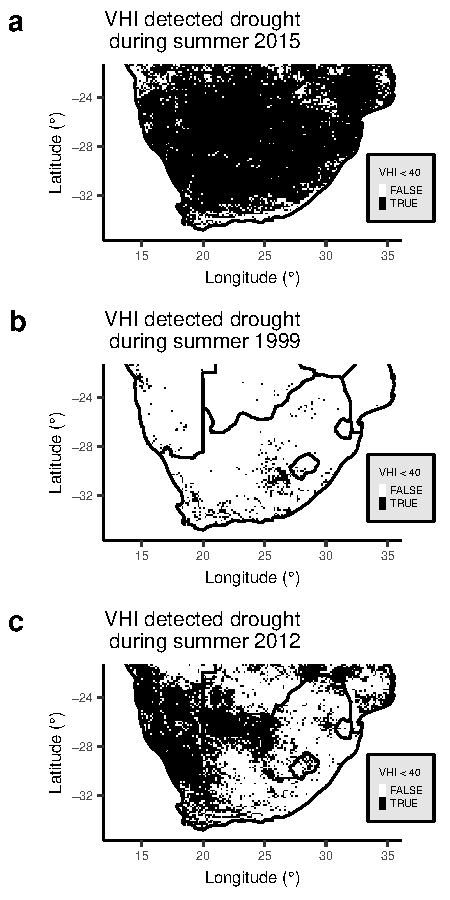
\includegraphics{../figures/maps_drought_examples.pdf}
\caption{\label{fig:mapsdroughtexamples}Example years experiencing contrasting degrees
of drought in southern Africa. Vegetative Health Index (VHI) values
below 40 indicate remotely sensed drought. Drought detection during
these years is validated by previously reported precipitation based
estimates of drought ocurrence (Monyela, 2017) which confirm that while
(a) 2015 was one of the worst drought years on record, (b) 1999 was one
of the wettest, and (c) 2012 was typical in terms of precipitation
patterns. It is worth noting that drought can be detected using the VHI
across ecosystems, including those inhabited by perennial rather than
annual \emph{Heliophila} species.}
\end{figure}





\begin{figure}
\centering
\includegraphics{../figures/speciesmaps.pdf}
\caption{\label{fig:speciesmaps}Maps of occurrence records for individual species.
Orange points indicate annual species. Blue points indicate perennial
species.}
\end{figure}


\end{document}
